\section{Bilanz und GuV im Accounting Equation Approach}

\textbf{Bilanz}: Momentaufnahme der wirtschaftlichen Situation eines Unternehmens zu einem bestimmten
Zeitpunkt
\begin{center}
	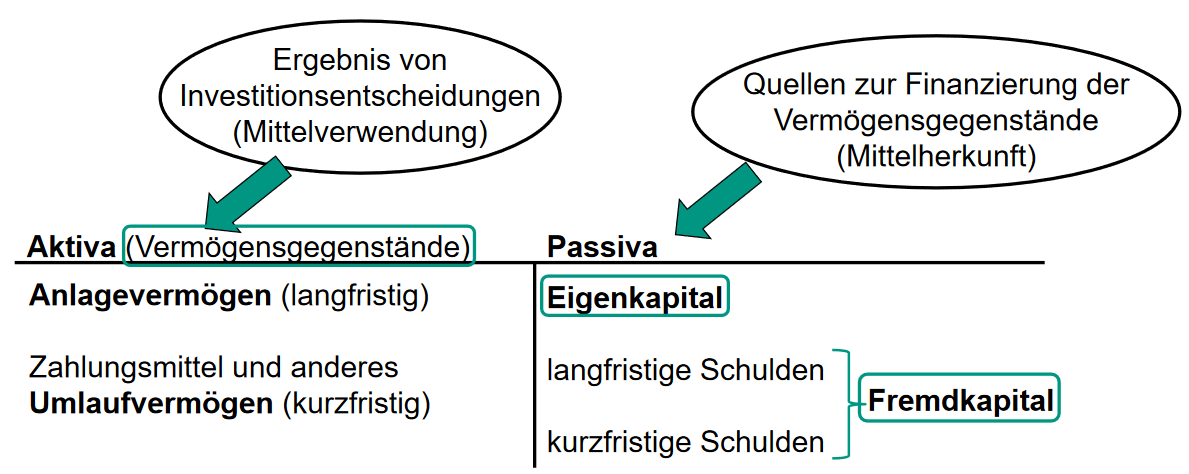
\includegraphics[width=0.7\textwidth]{images/bilanz.png}
\end{center}

\textbf{Vermögensgegenstände}: Repräsentieren zukünftige ökonomische Werte, die dem Unternehmen zufließen und zuverlässig in Geldeinheiten messbar sind
\begin{itemize}
	\item \textbf{Anlagevermögen} (langfristig): Sachanlagen, Finanzanlagen, Immaterielle Vermögensgegenstände, Aktive latente Steuern
	\item \textbf{Umlaufvermögen} (kurzfristig): Vorräte, Geleistete Anzahlungen, Forderungen, Wertpapiere, Liquide Mittel
	\item Vermögensgegenstände oft nur zu historischen Anschaffungskosten bewertet oder noch niedriger (Abschreibungen)
	\item Wertvolle Unternehmenseigenschaften, wie z.B. Humankapital (Fähigkeiten und Erfahrung der Mitarbeiter), Verträge über Großaufträge, Reputation und Marke bleiben unberücksichtigt!
	$\rightarrow$ Vorsichtsprinzip
\end{itemize}

\textbf{Fremdkapital}: 